\documentclass{beamer}
\usepackage{graphicx}

\usepackage{tikz}
\usetikzlibrary{trees}
\title{Das Ziegenproblem}
\usepackage{tikz}
\usetikzlibrary{trees}

%\usetheme{lucid}
\begin{document}
	\frame {
		\titlepage
	}
	\frame {
		\frametitle{Was ist das Ziegenproblem?}
		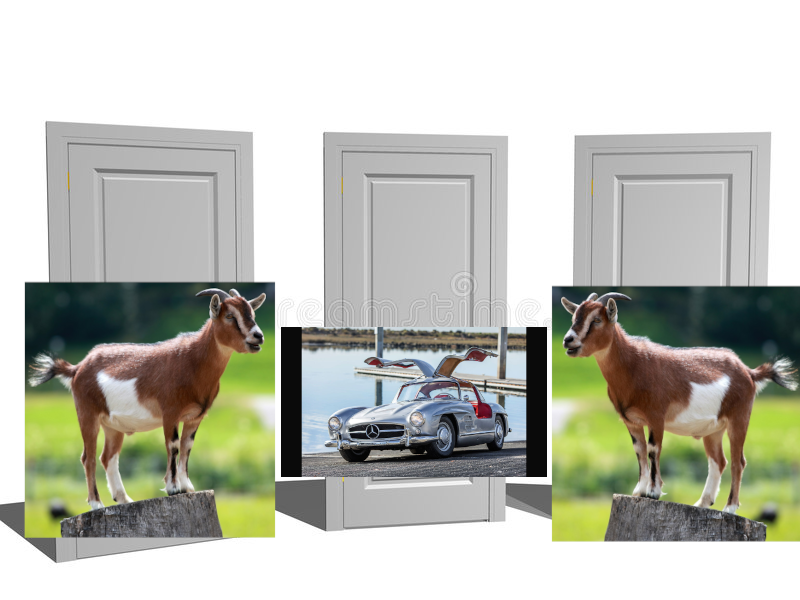
\includegraphics{dreitueren}
	}
	\frame{
		In wie vielen der 3 möglichen Konstellationen würde der Kandidat bei dieser Spielshow das Auto gewinnen, wenn...?
		\begin{itemize}
			\item der Spieler bei seiner Wahl bleibt?
			\item der Spieler zur letzten verbleibenden Tür wechselt?
		\end{itemize}
}

		\frame{
		\frametitle{Optimale Strategie?}
		Gibt es eine optimale Strategie, was meint ihr?
	}

	\frame{
		\frametitle{Simulation}
		Die Lösung: eine Simulation
	}

		\frame{
		\frametitle{Warum?}
		\small
		% Set the overall layout of the tree
\tikzstyle{level 1}=[level distance=3.5cm, sibling distance=3.5cm]
\tikzstyle{level 2}=[level distance=3.5cm, sibling distance=2cm]

% Define styles for bags and leafs
\tikzstyle{bag} = [text width=4em, text centered]
\tikzstyle{end} = [circle, minimum width=3pt,fill, inner sep=0pt]
\scalebox{0.75}{
\begin{tikzpicture}[grow=right, sloped]
\node[bag] {Wahl}
    child {
        node[bag] {Ziege 1}% This is the first of three "Bag 2"
        child {
                node[bag,fill=green!30!] {Wechsel}
                child {
                    node[bag,fill=green!30!] {Auto}
                }
            }
            child {
                node[bag,fill=yellow!30!] {Kein Wechsel}
                child{
                    node[bag,fill=yellow!30!] {Ziege 1}
                }
            }
    }
    child {
        node[bag] {Ziege 2}% This is the first of three "Bag 2"
        child {
                node[bag,fill=green!30!] {Wechsel}
                child {
                    node[bag,fill=green!30!] {Auto}
                }
            }
            child {
                node[bag,fill=yellow!30!] {Kein Wechsel}
                child{
                    node[bag,fill=yellow!30!] {Ziege 2}
                }
            }
    }
        child {
            node[bag] {Auto}
            child {
                    node[bag,fill=green!30!] {Wechsel}
                    child {
                        node[bag,fill=green!30!] {Ziege}
                    }
                }
                child {
                    node[bag,fill=yellow!30!] {Kein Wechsel}
                    child{
                        node[bag,fill=yellow!30!] {Auto}
                    }
                }
    };
\end{tikzpicture}
}
}

	\frame{
		\frametitle{Ausgedrückt in Ergebnismengen:}
		\begin{align*}
		\text{Ergebniraum:}\\
		\Omega &= \{Ziege1, Ziege2, Auto\}; \; |\Omega|= 3\\
		\text{Ergebnismenge mit Wechsel:}\\
		\Omega_{Wechsel} &= \{Ziege1, Ziege2\};\; |\Omega_{Wechsel}|=2\\
		\text{Ergebnismenge ohne Wechsel:}\\
		\Omega_{ohne Wechsel} &= \{ Auto \};\;|\Omega_{ohne Wechsel}|= 1\\
		\text{Daraus folgt: }\\
		P_{Wechsel} &= \frac{ |\Omega_{Wechsel}|}{|\Omega|}= \frac{2}{3}\\
		P_{ohne Wechsel} &= \frac{|\Omega_{ohne Wechsel}|}{|\Omega|}= \frac{1}{3}
		\end{align*}
	}
	\frame{
		\frametitle{Fortführung}
		Würdet ihr wechseln, wenn es n Türen gäbe und (n-2) davon geöffnet werden?
		}
	\frame{
		\frametitle{Quellen}
		\url{https://de.wikipedia.org/wiki/Hausziege#/media/Datei:Hausziege_04.jpg}\\
		\url{https://thumbs.dreamstime.com/b/drei-t\%C3\%BCren-1875644.jpg}\\
		\url{https://www.grin.com/document/214288}\\
		\url{https://www.pedocs.de/volltexte/2013/5807/pdf/UntWiss_2004_1_Krauss_Atmaca_Schueler_Einsicht.pdf}}

\end{document}
